\documentclass[10pt,twocolumn,letterpaper]{article}

\usepackage{cvpr}
\usepackage{times}
\usepackage{epsfig}
\usepackage{graphicx}
\usepackage{booktabs}
\usepackage{amsmath}
\usepackage{amssymb}

% Include other packages here, before hyperref.

% If you comment hyperref and then uncomment it, you should delete
% egpaper.aux before re-running latex.  (Or just hit 'q' on the first latex
% run, let it finish, and you should be clear).
\usepackage[breaklinks=true,bookmarks=false]{hyperref}

\cvprfinalcopy % *** Uncomment this line for the final submission

\def\cvprPaperID{****} % *** Enter the CVPR Paper ID here
\def\httilde{\mbox{\tt\raisebox{-.5ex}{\symbol{126}}}}

% Pages are numbered in submission mode, and unnumbered in camera-ready
%\ifcvprfinal\pagestyle{empty}\fi
\setcounter{page}{1}
\begin{document}

%%%%%%%%% TITLE
\title{SSD Object Detection Model for Blender Gestural Input Interface}

\author{Marzio Vallero\\
Politecnico di Torino\\
C.so Duca degli Abruzzi, 24, 10129, Torino, ITALY\\
{\tt\small marzio.vallero@studenti.polito.it}
% For a paper whose authors are all at the same institution,
% omit the following lines up until the closing ``}''.
% Additional authors and addresses can be added with ``\and'',
% just like the second author.
% To save space, use either the email address or home page, not both
}

\maketitle
%\thispagestyle{empty}

%%%%%%%%% ABSTRACT
\begin{abstract}
This paper aims at describing the steps required for the training of a custom purpose Object Detector neural network to be used as a mean of interaction for the 3D modeling software Blender. The first part will describe the generation of a custom dataset for training over hand gestures containing images of a single person, explaining techniques used to reduce as much as possible any bias due to this.\linebreak
This dataset will be then used to transfer learn a Single Shot Multibox Detector with Feature Pyramid architecture through Tensorflow's Object Detection API.
The results will be evaluated through training statistics and direct experimentation with the trained model, discussing about the approaches used and possible improvements.
Demos and code relative to this paper are available at the project's \href{https://github.com/MarzioVallero/ML-Based-Blender-Gestural-Input-Interface}{GitHub page}.
\end{abstract}

%%%%%%%%% BODY TEXT
\section{Introduction}
\begin{flushleft}
Most of modern era 3D software human-computer interfaces rely onto the usage of a mouse and a keyboard. This can prove to be a difficult task to learn, as this mean of manipulation can seems daunting and complex for newcomers.\linebreak
It has been proven already by Mavinkurve \etal~\cite{7814839} that Engineering Graphics are amongst the most difficult tasks to fully grasp for students and that 3D simulated environments improve their learning capabilities.\linebreak
This paper aims at detailing the steps required to create an object detection neural network able to recognize static hand gestures. Such network is a Single Shot Multibox Detector, as for the work of Liu \etal~\cite{ssd}, refined by Google Brain researchers Ghiasi \etal~\cite{ghiasi2019nasfpn}, and trained on Microsoft's COCO 17 dataset (Lin \etal~\cite{lin2015microsoft}). Its checkpoints are publicly available through the Tensorflow Model Garden, developed by Yu \etal~\cite{tensorflowmodelgarden2020}.\linebreak
At first, will be introduced the steps for the generation of a custom dataset for training, by applying data augmentation, also generating negative samples. This is done to reduce the bias due to the fact that it contains only images of the same person. This dataset will then be used to train through transfer learning (as per shown by Zhuang \etal~\cite{zhuang2020comprehensive}) a checkpoint of the SSD and discuss about training statistics and experimental results.\linebreak
The hereby proposed input interface could see applications as an instrument for learning (molecules, human body models or mechanical models) and as a mean of interaction in museums or during large-scale presentations.
\end{flushleft}

\section{Dataset}
\begin{flushleft}
The first step amounts to the generation of the custom dataset, justified by the fact that no current dataset exists containing all of the gestures required for this specific scope.
All the following steps are also described in depth in the Python notebook \href{https://github.com/MarzioVallero/ML-Based-Blender-Gestural-Input-Interface/blob/master/DatasetGeneration.ipynb}{DatasetGeneration.ipynb} as an additional support for understanding.\linebreak
The first step is responsible for the definition of the set of gestures and the set up of automated sample capture. After defining the number of images to collect for each object class, the frames are captured, then are automatically saved in separate directories according to their label of reference. For the sake of simplicity, it is recommended to produce for each label the same amount of samples and to insert a single gesture per frame. The effect of multiple, possibly different labels present in the same frame could be further investigated in future work.\linebreak
The amount of data at the network's disposal for training greatly impacts its ability to learn: for this very reason, data augmentation has been exploited in order to increase the number of available samples for the model's training, whilst trying to reduce the implicit bias due to the fact that the dataset contains only samples of the same individual. The data augmentation transformations used are horizontal/vertical stretching and zooming. Other data augmentation techniques could have caused shape overlaps between gestures and have thus been avoided. Negative samples have been introduced to reduce the amount of false positives registered by the network.\linebreak
Totally, 12 classes were defined, plus an extra unlabeled one for negative samples. For each class, 100 samples were produced.\linebreak
The main variance between sets of images for the same label lie in different spatial positions of the hand with respect to the frame and rotations of the wrist.\linebreak
It's important to note that a wider dataset for each gesure will increase variance, possibly increasing accuracy and the generalization capabilities of the final trained model.

The labeling process has been done with \textit{LabelImg}, a Python based graphic tool developed by Tzutalin~\cite{tzutalin2015labelimg} which allows for manual selection of one or multiple ROIs within each frame and label it according to a specific class.
This process produces, for each frame, an output \textit{.xml} file that embeds the coordinates of the region of interest and label of a specific frame. At the end of this process, it will have produced exactly one \textit{.xml} file for each sample in the dataset. The negative samples will have and empty \textit{.xml} file, generated by pressing \textit{Verify Image} on LabelImg's GUI.\linebreak

\begin{figure}[!h]
    \centering
    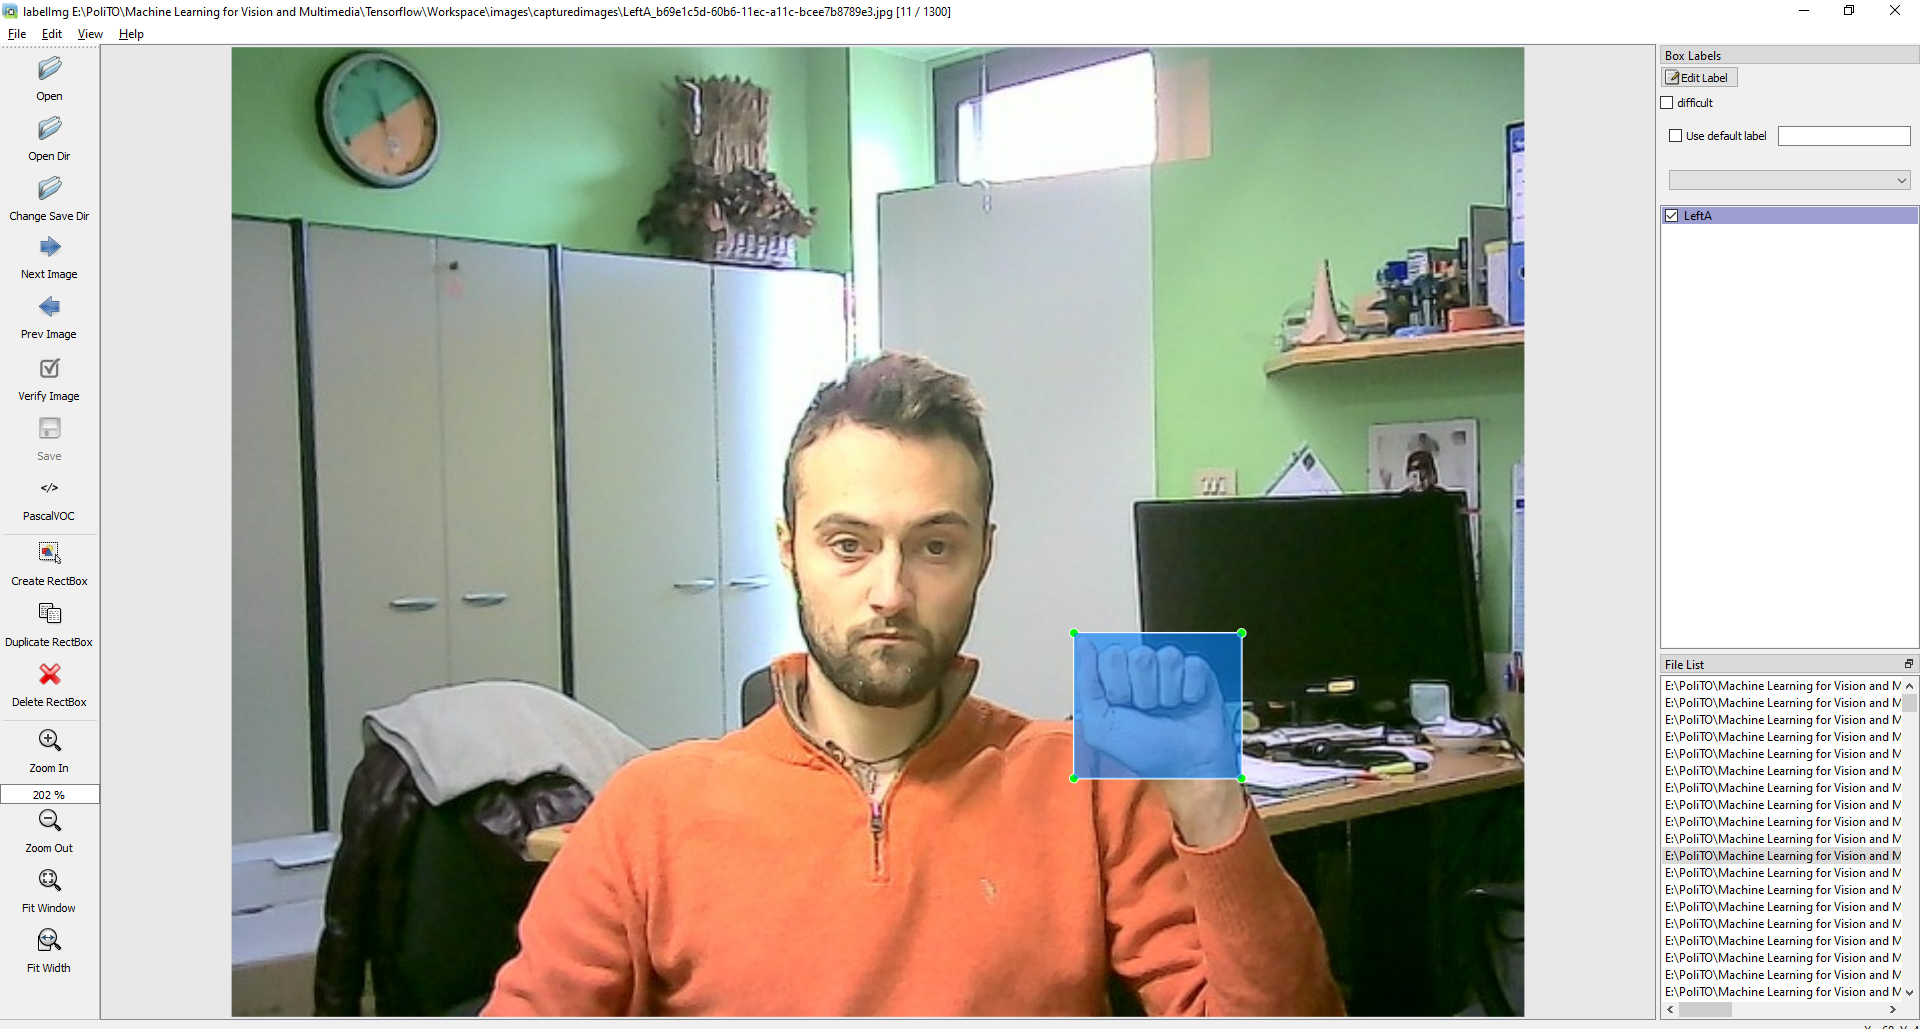
\includegraphics[width=0.5\textwidth]{resources/image/labelImgScreenshot.PNG} \caption{The LabelImg interface after drawing a bounding box around a gesture.}
\end{figure}

The final dataset thus contains $1300$ images representing the same person, on the same background, doing a total of 12 different gestures. It has been split into two partitions, with 25\% for validation and 75\% for training.
\end{flushleft}

\section{Methods}
\begin{flushleft}
The approach originally considered for the creation of an input interface for Blender was to build and train a RNN able to recognize actions from a video input. This however proved to be extremely inadequate in terms of usability, since repeating an action multiple times was the only way to produce incremental transformations through the interface. Moreover, the task of generating and labeling a custom dataset for such approach would have had a quite significant impact on the time available for the project's development. For this reason this approach was ultimately discarded.\linebreak
The second approach, which was later adopted, was to train an Object Detection network able to map continuous static input gestures to transformations in the 3D scene of Blender. The choice of using the SSD MobileNet V2 FPNlite network arised from its inherent state of the art characteristics: a very fast mean input processing time of $22$ ms, which suits perfectly the need to process video at 30 FPS from a webcam, which generates an image every $33.3$ ms, and its very high mAP score of $22.2$ over the COCO 17 dataset on which it was initially trained, as per the work of Yu \etal~\cite{tensorflowmodelgarden2020} (at \textit{models/research/object\_detection/g3doc/tf2\_detection\_zoo.md}).\linebreak
This approach moreover allowed for the exploitation of transfer learning to retrain a pre-existing model, improving considerably the time required for training.
\end{flushleft}

\subsection{Architecture}
\begin{flushleft}
The chosen model was originally developed by Ghiasi \etal~\cite{ghiasi2019nasfpn} and aimed at improving over current hand-crafted CNNs, defining a better architecture of feature pyramid networks for object detection, called NAS-FPN.
The model's architecture has been later improved in the work of Sandler \etal~\cite{sandler2019mobilenetv2}, which will be summarized in the following subsection.
The main changes which have been applied to such model are the removal of the \textit{random\_horizontal\_flip} data augmentation layer and the reduction of total training steps, justified by the fact that the dataset used is much smaller with respect to COCO 17 and thus boasts less features to be learnt.\linebreak
The basic building block introduced in Sandler \etal's paper is a bottleneck depth-separable convolution layer with residuals, whose structure is shown in \hyperref[figure2]{Figure 2}.

\begin{figure}[!h]
    \centering
    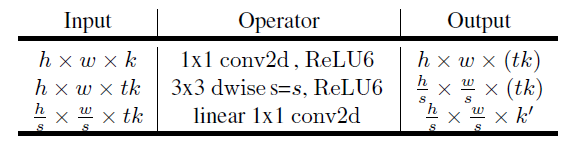
\includegraphics[width=0.5\textwidth]{ML SSD project/resources/image/MoblieNetV2Table1.png} \caption{Bottleneck residual block transforming from k to k' channels, with stride s, and expansion factor t.}
\end{figure}
\label{figure2}

The general architecture of the model contains an initial fully convolutional layer with 32 filters, followed by 19 residual bottleneck layers, as shown in \hyperref[figure3]{Figure 3}. The kernel size is 3 × 3, and dropout and batch normalization layers are used during training.

\begin{figure}[!h]
    \centering
    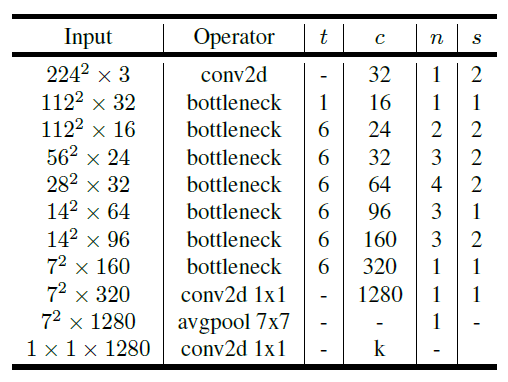
\includegraphics[width=0.5\textwidth]{resources/image/MoblieNetV2Table2.png} \caption{The full model's architecture. Each line represents n repetitions of the same layer. All layers feature the same number of channels c. The first sequence layer has stride s, whilst the others have stride 1.}
\end{figure}
\label{figure3}

This architecture is then wrapped between six \textit{bottom\_up\_conv\_2d} layers and a \textit{FeatureMap} layer, as shown in \hyperref[figure4]{Figure 4}.
As it can be seen, this version of the model features $2,223,872$ trainable parameters and $34,112$ non-trainable ones.\linebreak

\begin{figure}[!h]
    \centering
    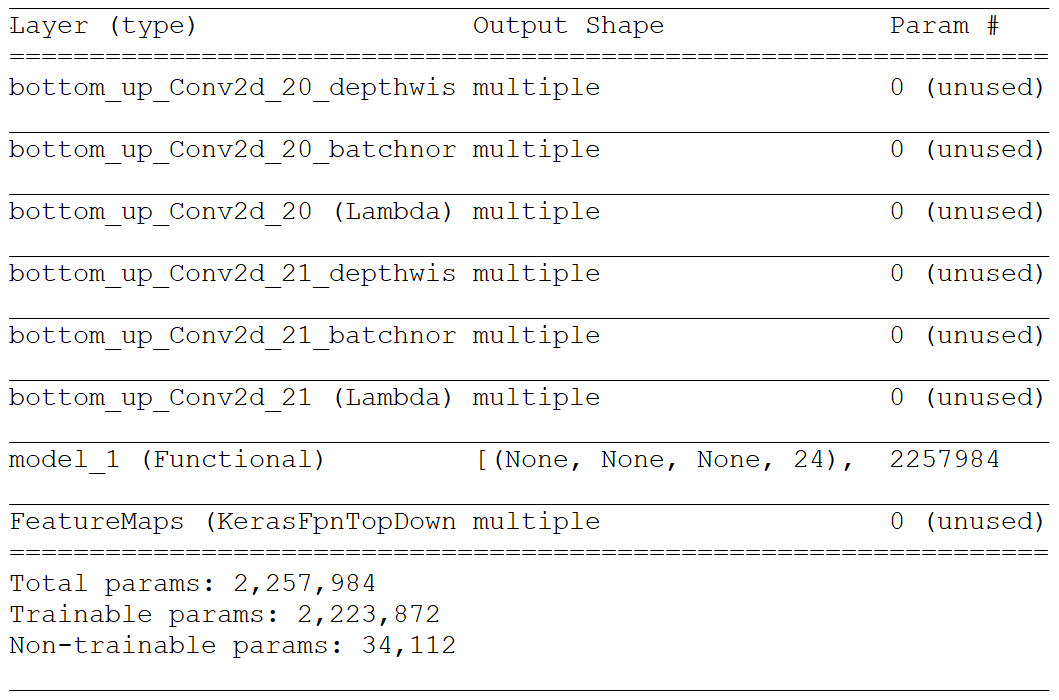
\includegraphics[width=0.5\textwidth]{ML SSD project/resources/image/architecture.PNG} \caption{The wrapped model's architecture, complete with parameters.}
\end{figure}
\label{figure4}

\end{flushleft}
\subsection{Hyperparameters}
\begin{flushleft}
The loss used for training is split into four elements: classification, localization, regularization and total loss.
Classification loss refers to the model's ability to correctly predict an object's class and uses as loss function a weighted sigmoid focal, with gamma equal to 2 and alpha equal to 0.25.
Localization loss refers to the ability to find the position of the bounding box of an object inside the input image and uses as loss function a weighted smooth L1 function.
Regularization loss is an additional loss generated by the L2 regularization function, which gets added to the network's loss and used to optimize over the sum of the other two. This method is used to help the optimization algorithm to generalize better over the dataset.
The total loss represents the sum of these three previous losses and gives a top-down view of the model's training performance.\linebreak
The model's live performance has then been evaluated through the \href{https://github.com/MarzioVallero/ML-Based-Blender-Gestural-Input-Interface/blob/master/ModelTest.ipynb}{ModelTest.ipynb} notebook, checking the predicted labels superimposed over the input frames.\linebreak
To boost the model's prediction accuracy, HSV skin tone thresholding has been applied to remove most false positives and stabilizing the model's performance in the wild. The results were extremely encouraging and thus this pre-processing step has been mantained in the final evaluation script.

\end{flushleft}

\section{Experiments}
\begin{flushleft}
All the models have been trained onto a machine equipped with an \textit{Intel i5-11600K} CPU, 32 GB of DDR4 3600 MHz RAM and accelerated through an \textit{NVidia GeForce RTX 2060 6GB} GPU.
\end{flushleft}
\subsection{Training}
\begin{flushleft}
The first training has been done over $20000$ steps, with a batch size of $8$, totaling $164$ epochs, and required over two hours to complete: this produced a model with a final Total Loss of $0.12568491$, still too high to provide stable predictions. Testing this checkpoint in fact proved to be unfeasible, as it was not able to recognize almost anything at all during the evaluation phase.
The training has then been resumed for another $20000$ steps, requiring another two hours and a half. The final Total Loss came out to be $0.09876089$, which is a great improvement over previous iterations. However, testing the model live immediately gave rise to bounding box detection issues and general inaccuracy of the predictions, without much generalization capabilities. Moreover, since the network during training internally performed horizontal flips for data augmentation, the left and right hand gestures got often swapped or overlapped. To boost the accuracy of the network, its input gets thresholded using an HSV profile, customizable to better suit each user.
The hand swapping issue, has been solved by retraining the model from scratch whilst removing the horizontal flip data augmentation layer, this time with a batch size of $16$, totaling $656$ epochs. This last training required only four hours and a half to complete, suggesting that the GPU's hardware characteristics were not well exploited previously.
The training statistics for this last model are shown in \hyperref[figure5]{Figure 5}.

\begin{figure}[!h]
    \centering
    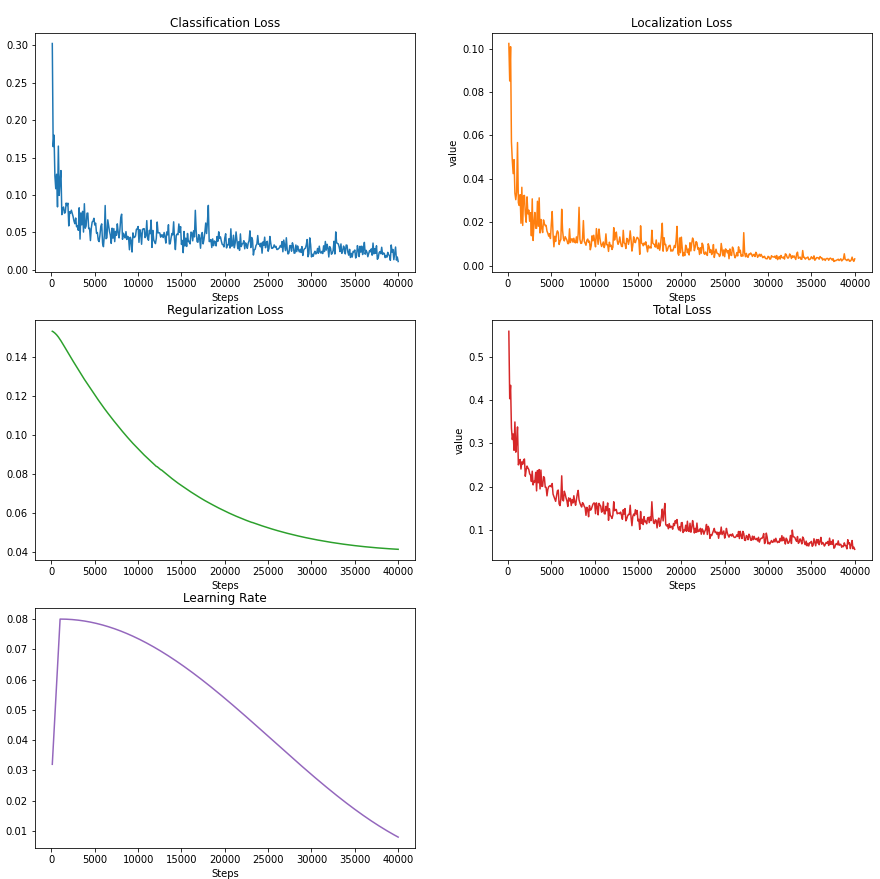
\includegraphics[width=0.5\textwidth]{ML SSD project/resources/image/statistics.PNG} \caption{All losses and learning rate statistics for the 40000 steps model trained without the horizontal flip data augmentation layer. From top left to bottom right: Classification Loss, Localization Loss, Regularization Loss, Total Loss and Learning Rate.}
\end{figure}
\label{figure5}

\end{flushleft}
\subsection{HSV thresholding}
\begin{flushleft}
The role of the HSV thresholding preprocessing step plays an impactful role on the model's ability to process the input frames. Despite the fact that the dataset contains images with hands in different spatial positions over a complex background, the model sometimes produces FP, detecting a gesture where there is none. This may be due to the fact that the whole dataset contains the same static background, or that some of the features learnt by the network are edge bound and some objects happen to fit partially those feature requirements. However, after a thresholding and opening transformation, most of the background contains no data, as shown in \hyperref[figure6]{Figure 6}, and thus gives to the model less room for error in evaluating gestures. To prove its beneficial effects, an ablation study has been conducted, whose results can be seen in \hyperref[table1]{Table 1}.
Some classes benefit very little from the thresholding procedure, like \textit{LeftA} and \textit{RIndexFront}. Some obtain a great improvement, like \textit{RThumbBack} and \textit{RIndexRight}, while most of the classes show a 2-5\% improvement on average. The \textit{LeftO}, \textit{LeftV} and \textit{RIndexDown} get an average 2\% worsening, which however gets outweighted by the improvements in detecting the other nine classes. As such, the preprocessing step has been kept as part of the model.

\begin{figure}[!h]
    \centering
    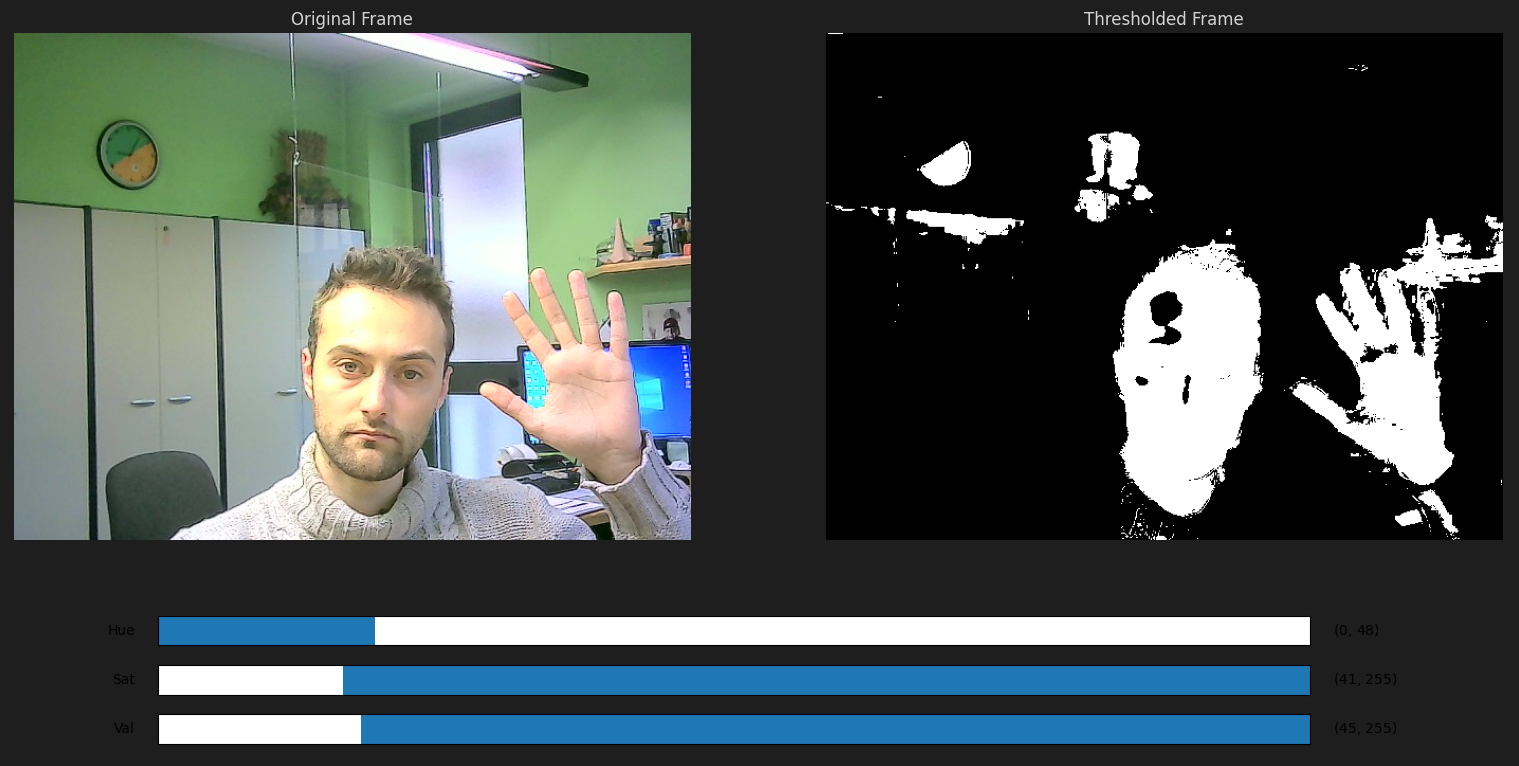
\includegraphics[width=0.5\textwidth]{ML SSD project/resources/image/thresholding.PNG}
    \caption{The effect of thresholding, as seen thorugh the \textit{\href{https://github.com/MarzioVallero/ML-Based-Blender-Gestural-Input-Interface/blob/master/CreateHSVProfile.py}{CreateHSVProfile.py}} script.}
\end{figure}
\label{figure6}

\end{flushleft}
\subsection{Results}
\begin{flushleft}
All the performance metrics hereby presented are based on the work of Padilla \etal~\cite{electronics10030279}.\linebreak
The precision to recall curves for the 12 classes have been computed for two different values of Intersection Over Union percentages: 50\% and 80\%. This has been done as a way to provide insight over the model's stability in correctly localizing a gesture.\linebreak
In the $IOU=50$ curves, shown in \hyperref[figure7]{Figure 7}, it's clear to see that the model is able to yield exceptional precision over all the classes with respect to the recall, with the \textit{LeftA} and \textit{RIndexRight} boasting a AP score of $1.0$ and most of the other classes following closely to the same result. The two worst performing classes are \textit{RIndexUp} and \textit{RThumbBack}, respectively with an AP score of $0.9217$ and $0.9242$, which are still extremely good results. All the \textit{PASCAL} AP scores are listed in \hyperref[table1]{Table 1}.

\def\arraystretch{1.2}%
\begin{table*}[!h]
    \begin{center}    
        \begin{tabular}{l|r|r|r|r}
        \hline
        \multicolumn{5}{c}{AP scores}\\
        \hline
        \hline
        \texttt{Classes} & $AP_{50}$ \texttt{with HSV} & $AP_{80}$ \texttt{with HSV} & $AP_{50}$ \texttt{raw} & $AP_{80}$ \texttt{raw}\\
        \hline
        \texttt{LeftA} & \textbf{1.0} & 0.4105 & \textbf{1.0} & \textbf{1.0} \\
        \hline
        \texttt{LeftL} & \textbf{0.9933} & 0.5018 & 0.8775 & 0.7950 \\
        \hline
        \texttt{LeftO} & 0.9843 & 0.3903 & \textbf{1.0} & 0.7963 \\
        \hline
        \texttt{LeftOpenHand} & \textbf{0.9890} & 0.8517 & 0.9600 & 0.4324 \\
        \hline
        \texttt{LeftV} & 0.9453 & 0.1717 & \textbf{0.9855} & 0.6535 \\
        \hline
        \texttt{RClearC} & \textbf{0.9969} & 0.2654 & 0.9892 & 0.6420 \\
        \hline
        \texttt{RIndexDown} & 0.9694 & 0.6183 & \textbf{0.9938} & 0.9087 \\
        \hline
        \texttt{RIndexFront}  & \textbf{0.9846} & 0.1852 & 0.9823 & 0.5765 \\
        \hline
        \texttt{RIndexLeft}  & \textbf{0.9969} & 0.4494 & 0.9699 & 0.7648 \\
        \hline
        \texttt{RIndexRight}  & \textbf{1.0} & 0.0242 & 0.6334 & 0.1389 \\
        \hline
        \texttt{RIndexUp} & \textbf{0.9217} & 0.5382 & 0.8147 & 0.4875\\
        \hline
        \texttt{RThumbBack} & \textbf{0.9242} & 0.0240 & 0.3184 & 0.2426 \\
        \hline
        \end{tabular}
    \end{center}
    \caption{The AP scores among the 12 classes and both IOU values. The highest AP scores for each class are in bold.}
    \label{table1}
\end{table*}

\begin{figure}[!h]
    \centering
    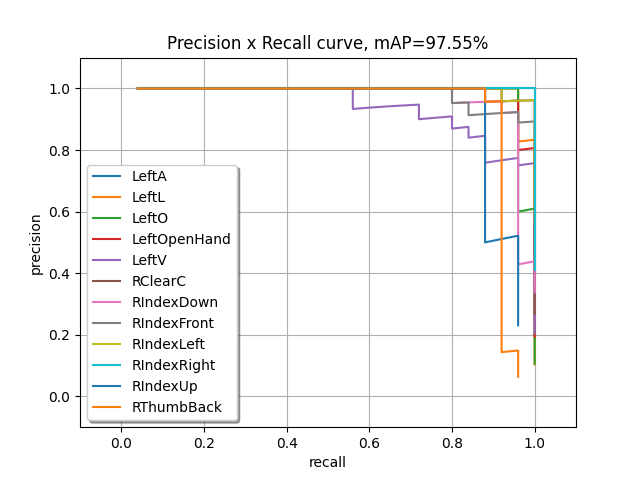
\includegraphics[width=0.5\textwidth]{ML SSD project/resources/image/all_classes_IOU50.png}
    \caption{The precision to recall curves for all the 12 proposed gesture classes, with IOU = 50 and HSV thresholding.}
\end{figure}
\label{figure7}

The steeper requirement of an $IOU=80$ value is reflected onto the precision to recall curves shown on \hyperref[figure8]{Figure 8}. The best performing class is \textit{LeftOpenHand}, which yields an encouraging AP value of $0.8517$, suggesting for it to be the most stable class. However, most of the other classes make the model fall short of the expectations, with only six other classes boasting an AP score sufficiently close or greater than $0.4$. The two worst performing classes are \textit{RIndexRight} and \textit{RThumbBack}, both with a AP score close to $0.0240$, suggesting that these two classes tend to be harder to correctly localize and detect for the model.
\begin{figure}[!h]
    \centering
    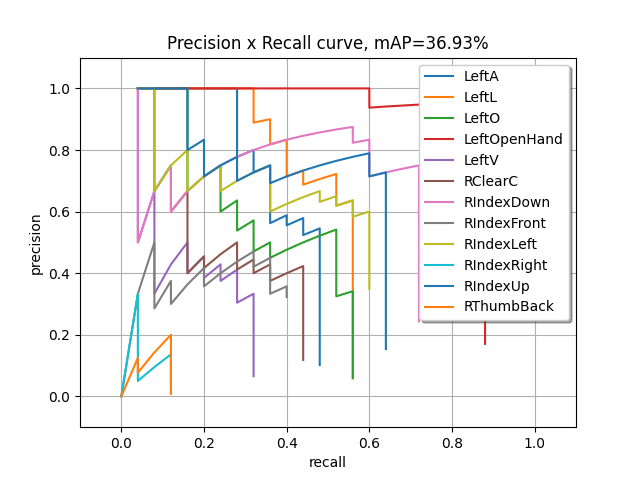
\includegraphics[width=0.5\textwidth]{ML SSD project/resources/image/all_classes_IOU80.png}
    \caption{The precision to recall curves for all the 12 proposed gesture classes, with IOU = 80 and HSV thresholding.}
\end{figure}
\label{figure8}

Over all the classes, the model boasts the following \textit{COCO} metrics. The $AP_{50}$ has a value of $0.9757$, in line with its relative \textit{PASCAL} AP metric. The $AP_{75}$ has a value of $0.5704$, whilst the overall $AP$ has a slightly smaller value of $0.5645$. This skew between the \textit{COCO} and \textit{PASCAL} metrics suggests that the model's performance is promising and that the $IOU=80$ value is a requirement too steep to be satisfied as per the current architecture of the network. Morever, the proposed set of gestures proved to contain common features between classes, as the number of FP explodes as soon as we try to consider lower confidence predictions.

\end{flushleft}

\section{Conclusions}
\begin{flushleft}
The process of producing and understanding the model presented in this paper has been multi-faceted and long, however it also proved to be a very formative experience.\linebreak
The generation of the dataset has been a quite daunting task, requiring multiple days of work just for capturing and labeling. Moreover, the expansion of the dataset to include also negative samples to feed to the network resulted into a better generalization of the gesture features, reducing by a significant margin the false positives due to predicting gestures where there are none. In fact, one of the most common pitfalls in these kinds of applications is the false prediction of a hand gesture on the user's face, which in our case has been mitigated quite well.\linebreak
Setting up the \textit{pipeline.config} file proved to be a challenging task too, due to the required installation of the Tensorflow Object Detection API, which brought in many versioning issues deriving from Tensorflow 1 and 2 incompatible calls among the \textit{Tensorflow/models} submodule's scripts. In the end, parts of those scripts had to be modified in order to account for updates in Tensorflow's API.\linebreak
The analysis of the \textit{pipeline.config} file also gave insight about the inner workings of the model, opening the possibility for tinkering around hardware specific definitions to improve training performance (like the batch size, which has been found to boast better performance at value 16) and removing components which were working against our needs.\linebreak
The model's generalization capabilities over the single-person dataset proved to be extremely promising when live-tested onto different people. The model expects a certain shape and orientation, thus incorrect gestures due to different individual's interpretation still get unrecognized, though gestures which try to resemble more the original dataset end up being recognized with no issue and a high confidence of around 90\%. This requires some of effort from the user's side to work, however it's believable for it to be a quite encouraging result given the amount of data available. This aspect could be improved by generating a bigger dataset with higher user variance, especially in terms of hand morphology and skin tone, and consequently training for a higher number of steps.\linebreak
It's important to note how a thorough study of a new gesture set could improve the model's performnace in future works, as some of the gestures shared morphological features which caused the model to produce more FP than expected.
The thresholding external preprocessing step, originally implemented following Nikam \etal~\cite{7916786}'s work as a \textit{YCbCr} thresholding, proved to boast low masking capabilities with respect to skin tone. It has later been changed to the current \textit{HSV} thresholding script, as allows for more precise masking for \textit{in-the-wild} environments.\linebreak
In conclusion, the results of this paper are to be considered significant, in that they provide insight over the techniques and approaches to be used to produce gestural input interfaces through the exploitation of state of the art object detector neural networks.\linebreak
\end{flushleft}

\pagebreak
{\small
\bibliographystyle{ieee_fullname}
\bibliography{egbib}
}

\end{document}
